\documentclass[12pt]{beamer}
\usepackage[T2A]{fontenc} 
\usepackage[utf8]{inputenc} 
\usepackage{algorithm}
\usepackage{algorithmic}
\usepackage{makecell}
\usepackage[english, ukrainian]{babel} 
\mode<presentation>{
	\usetheme{CambridgeUS}
    \setbeamercovered{transparent}
}
%% preamble
\title{Ієрархічні матриці у методі граничних елементів}
\author{Солук Олена}
\date[ 2019]
{\large{Львівський національний університет імені І.Франка}}
\begin{document}
\begin{frame}
	\titlepage
\end{frame}
%% normal frame
\begin{frame}{Зміст}
\begin{block}{}
	1. Кластерне дерево i блочне кластерне дерево.\\
	2. Умова допустимості.\\
	3. Означення $\mathcal{H}$-матриці.\\
	4. Модельна задача.\\
	5. Чисельні експерименти.
\end{block}	
\end{frame}


\begin{frame}{Кластерне дерево}
	\begin{block}{}
		$$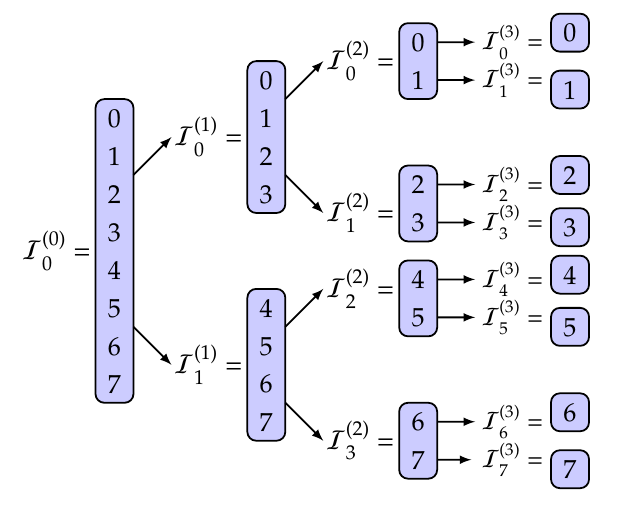
\includegraphics[scale=0.48]{1_0}$$
	\end{block}
\end{frame}
\begin{frame}
\frametitle{Block Cluster Tree}
	\begin{block}{Означення}
	Нехай $\mathbb{T}_{I}$ і $\mathbb{T}_{J}$ - кластерні дерева над множинами індексів $I$ та $J$ відповідно. Кластерне дерево $\mathbb{T}_{I\times J}=\mathbb{T}_{\mathbb{T}_{I}\times \mathbb{T}_{J}}=(V,E)$ називається блочне кластерне дерево над добутком множини індексів $I\times J$, якщо $\forall v\in V$ виконуються наступні умови:
		\begin{enumerate}
			\item[-] $\mathbb{T}^{(0)}_{I\times J}=I\times J$
			\item[-] Якщо $v\in \mathbb{T}^{(l)}_{I\times J}$, то існують $\tau \in \mathbb{T}^{(l)}_I$ i $\sigma \in \mathbb{T}^{(l)}_J$ такі, що $v=\tau \times \sigma$.
			\item[-] Для синів $v=\tau \times \sigma$, де  $\tau \in \mathbb{T}_I$ i $\sigma \in \mathbb{T}_J$ виконується
			\newline
			S(v)=$\begin{cases}
			$\O,$\text{якщо $S(\tau)=\O$ або $S(\sigma)=\O$}\\
			$$\{\tau^{\prime}\times\sigma^{\prime} : \tau^{\prime} \in S(\tau),\sigma^{\prime} \in S(\sigma)\}$,$\text{інакше}
			\end{cases}$
		\end{enumerate}
	\end{block}
\end{frame}

\begin{frame}
\frametitle{Умова допустимості}
	 Ми будемо використовувати стандартну умову допустимості в такому вигляді
		\newline
		$$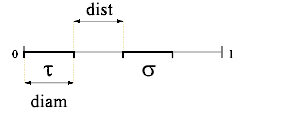
\includegraphics{1_2}$$
		$$diam(\tau)\le dist(\tau,\sigma)$$
	
\end{frame}

\begin{frame}{Приклад побудови блочного кластерного дерева}
	\begin{block}{}
		\centering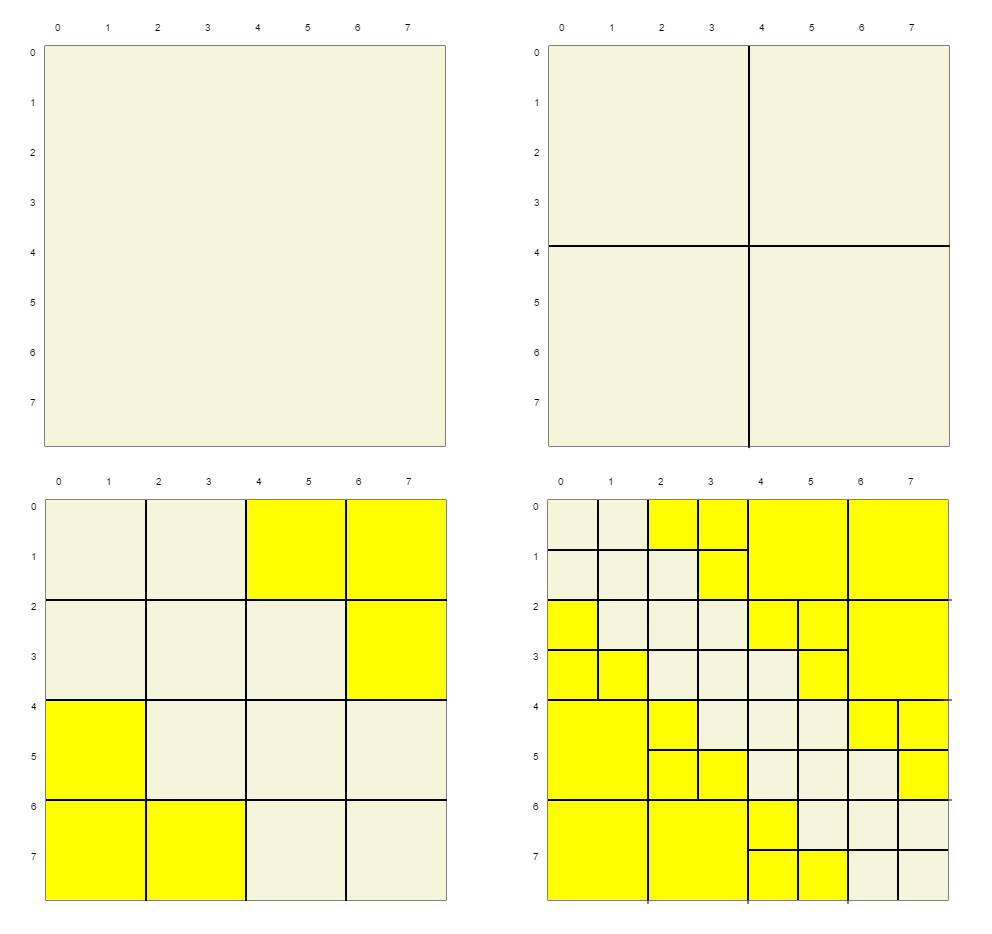
\includegraphics[scale=0.27]{1_3}
	\end{block}
\end{frame}
\begin{frame}
\frametitle{Означення $\mathcal{H}$-матриці}
	\begin{block}{Означення}
		Нехай $\mathbb{T}_{I\times I}$ - блочне кластерне дерево над множиною індексів $I$. Означаємо множину $\mathcal{H}$-матриць як
			$$\mathcal{H}(\mathbb{T}_{I\times I},k):=\{M\in\mathbb{R}^{I\times I}|rank(M|_{t\times s})\le k \text{ для всіх}$$ $$\text{допустимих листків } t\times s \text{ дерева } \mathbb{T}_{I\times I} \}$$
	\end{block}
\end{frame}
\begin{frame}{Модельна задача}
	\begin{block}{}
		Нехай задано функцію $F:[0,1]\rightarrow \mathbb{R}$. Шукаємо функцію $u:[0,1]\rightarrow \mathbb{R}$, яка задовільняє наступне інтегральне рівняння: $$\int_{0}^{1}\ln|x-y|u(y)dy=F(x), x\in[0,1] \eqno(1)$$
			де $g(x,y)=\ln|x-y|$ називається ядром інтегрального рівняння
	\end{block}
	\begin{block}{Метод Гальоркіна}
	$V_n=span\{\varphi_0,\dots,\varphi_{n-1}\}$
		
		$$\int_{0}^{1}\int_{0}^{1}\varphi_i(x)\ln|x-y|u(y)dydx=\int_{0}^{1}\varphi_i(x)F(x)dx\eqno(2) $$
		
		
	\end{block}
\end{frame}
\begin{frame}{}
	\par Потрібно знайти $u_n$ в просторі $V_n$:
			$$u_n=\sum_{j=0}^{n-1}u_j\varphi_j\eqno(3)$$
			таке, що вектор коефіцієнтів $u$ є розв'язком лінійної системи $$Gu=f$$
			$$G_{ij}=\int_{0}^{1}\int_{0}^{1}\varphi_i(x)\ln|x-y|\varphi_j(y)dydx\eqno(4)$$ 
			$$f_i=\int_{0}^{1}\varphi_i(x)F(x)dx$$
\end{frame}
\begin{frame}
	\begin{block}{}
	Базисні функції визначені як
		\newline 
		\begin{equation*}
		\varphi_i(x)=\begin{cases}
					1,\quad\text{якщо $\frac{i}{n}\le x< \frac{i+1}{n}$}\\
					0,\quad\text{інакше}
					\end{cases}
		\end{equation*}
	\end{block}
	\begin{block}{} 	$$\tilde{G}_{ij}=\int_{0}^{1}\int_{0}^{1}\varphi_i(x)\tilde{g}(x,y)\varphi_j(y)dydx = $$
		$$\int_{0}^{1}\int_{0}^{1}\varphi_i(x)\sum_{v=0}^{k-1}g_v(x)h_v(y)\varphi_j(y)dydx $$
		$$=\sum_{v=0}^{k-1}(\int_{0}^{1}\varphi_i(x)g_v(x)dx)(\int_{0}^{1}\varphi_j(y)h_v(y)dy)$$
	\end{block}
\end{frame}

\begin{frame}
\frametitle{Наближення низького рангу блоків матриці}
	\begin{block}{}
		$$\tilde{G}_{ij}=\int_{0}^{1}\int_{0}^{1}\varphi_i(x)\tilde{g}(x,y)\varphi_j(y)dydx = $$
		$$\int_{0}^{1}\int_{0}^{1}\varphi_i(x)\sum_{v=0}^{k-1}g_v(x)h_v(y)\varphi_j(y)dydx $$
		$$=\sum_{v=0}^{k-1}(\int_{0}^{1}\varphi_i(x)g_v(x)dx)(\int_{0}^{1}\varphi_j(y)h_v(y)dy)$$
	\end{block}
	\begin{block}{Факторизований вигляд підматриці}
		$$G|_{t\times s}=AB^\top,\quad A\in\mathbb{R}^{t\times\{0,\dots,k-1\}},\quad B\in\mathbb{R}^{s\times\{0,\dots,k-1\}}$$
			$$A_{iv}:=\int_{0}^{1}\varphi_i(x)g_v(x)dx, \quad B_{jv}:=\int_{0}^{1}\varphi_j(y)h_v(y)dy\eqno(5)$$
	\end{block}
\end{frame}
\begin{frame}
\frametitle{}
	\begin{block}{Недопустимі листки}
	$$\tilde{G_{ij}}:=\int_{0}^{1}\int_{0}^{1}\varphi_i(x)\ln|x-y|\varphi_j(y)dydx$$$$=\int_{i/n}^{(i+1)/n}\int_{j/n}^{(j+1)/n}ln|x-y|dydx$$
	\end{block}
	\begin{block}{Допустимі листки}
	$$\tilde{G}|_{t\times s}:=AB^\top$$
		$$A_{iv}:=\int_{i/n}^{(i+1)/n}(x-x_0)^vdx$$
		\begin{equation*}
			B_{jv}:=\begin{cases}
						(-1)^{v+1}v^{-1}\int_{j/n}^{(j+1)/n}(x_0-y)^{-v}dy,\quad\text{якщо $v>0$}\\
						\int_{j/n}^{(j+1)/n}\ln|x_0-y|dy,\quad\text{якщо $v=0$}
					\end{cases}
		\end{equation*}
	\end{block}
\end{frame}
\begin{frame}{Чисельні експерименти}
	\begin{block}{Приклад 1}
		$$\int_{0}^{1}\log|x-y|u(y)dy =\frac{2x^2\log|x|-2\log|x-1|(x^2-1)-2x-1}{4}$$
		$$u^*(x)=x$$
			\begin{table}[ht]
			\centering 
			\scalebox{0.7}{
			\begin{tabular}{c c c c c c } % centered columns (4 columns)
				\hline\hline %inserts double horizontal lines
				
				\diaghead(-2,1){aaaaaaa}{n}{k} & 1 & $\frac{n}{4}$ & $\frac{n}{2}$  & $\frac{3n}{4}$ & n \\ [0.5ex] % inserts table
				%heading
				\hline % inserts single horizontal line
				4 & 0.142393 & 0.142393 & 0.1423937 & 0.1423937 &0.1423937 \\ % inserting body of the table
				16 & 0.035737 & 0.0357365 & 0.0357365 &0.0357365&0.0357365\\
				64 & 0.00894708 &0.00894237 & 0.00894237 &0.00894237&0.00894237\\
				256 & 0.0022506 & 0.00223609 & 0.00223609 &0.00223609&0.00223609\\
				1024 & 7.7118E-4 & 5.590532E-4 & 5.59053E-4 &5.59053E-4&5.5905321665E-4\\ [1ex] % [1ex] adds vertical space
				\hline %inserts single line
			\end{tabular}
		}
			\label{table:nonlin} % is used to refer this table in the text
		\end{table}
	 \end{block}
\end{frame}
\begin{frame}{}
 	\begin{block}{Приклад 2}
 		$$\int_{0}^{1}\log|x-y|u(y)dy=-\dfrac{\left(12x^3-18x^2\right)\ln\left(\left|x\right|\right)-12\ln\left(\left|x-1\right|\right)x^3+}{36}$$$$\dfrac{+\left(18\ln\left(\left|x-1\right|\right)-12\right)x^2+12x-6\ln\left(\left|x-1\right|\right)+5}{36}$$
 		$$u^*(x)=x(1-x)$$
 		\begin{table}[ht]
 			\centering 
 			\scalebox{0.7}{
 			\begin{tabular}{c c c c c c } % centered columns (4 columns)
 				\hline\hline %inserts double horizontal lines
 				
 				\diaghead(-2,1){aaaaaaa}{n}{k} & 1 & $\frac{n}{4}$ & $\frac{n}{2}$  & $\frac{3n}{4}$ & n \\ [0.5ex] % inserts table
 				%heading
 				\hline % inserts single horizontal line
 				4 & 0.09689281 &0.09689281 & 0.09689281 & 0.09689281 &0.09689281 \\ % inserting body of the 
 				16 & 0.03246286 & 0.032463147 & 0.032463147 &0.03246314722&0.03246314722\\
 				64 & 0.00873409 &0.008736689 & 0.008736689 &0.008736689&0.008736689\\
 				256 & 0.002215192 & 0.0022232 & 0.0022232 &00.0022232047&0.00222320\\
 				1024 & 5.40425E-4 & 5.58247E-4 & 5.58247E-4 &5.582473E-4&5.582473E-4\\ [1ex] % [1ex] adds vertical space
 				\hline %inserts single line
 			\end{tabular}
 		}
 			\label{table:nonlin} % is used to refer this table in the text
 		\end{table}	
 	\end{block}
\end{frame}
\begin{frame}{}
\begin{block}{Приклад 3}
		$$\int_{0}^{1}\log|x-y|u(y)dy = x\log|x|+(1-x)\log|1-x|-1$$
	$$u^*(x)=1$$
	\begin{table}[ht]
		\centering 
		\scalebox{0.7}{
			\begin{tabular}{c c c c c c } % centered columns (4 columns)
				\hline\hline %inserts double horizontal lines
				
				\diaghead(-2,1){aaaaaaa}{n}{k} & 1 & $\frac{n}{4}$ & $\frac{n}{2}$  & $\frac{3n}{4}$ & n \\ [0.5ex] % inserts table
				%heading
				\hline % inserts single horizontal line
				4 & 8.881784E-16 & 8.881784E-16 & 8.8818E-16 & 8.8818E-16 &8.8818E-16 \\ % inserting body of the table
				16 & 1.99770E-6 & 2.02060E-14 & 2.020606E-14 &2.020606E-14&2.042810E-14\\
				64 & 1.9708842E-5 & 4.993783E-13 & 4.9938E-13 &4.993783E-13&5.140338E-13\\
				256 & 7.34135E-5 & 1.18067E-11 & 1.18067E-11 &1.18067E-11&1.176681E-11\\
				1024 & 2.3177027E-4 & 2.04782E-10 & 1.98478E-10 &1.9847878E-10&2.00121E-10\\ [1ex] % [1ex] adds vertical space
				\hline %inserts single line
			\end{tabular}
		}
		\label{table:nonlin} % is used to refer this table in the text
	\end{table}	
\end{block}
\end{frame}
\begin{frame}
	\begin{center}
		\Huge{Дякую за увагу!}
	\end{center}
\end{frame}

\end{document}
